\begin{figure}[thb]
  \begin{center}
    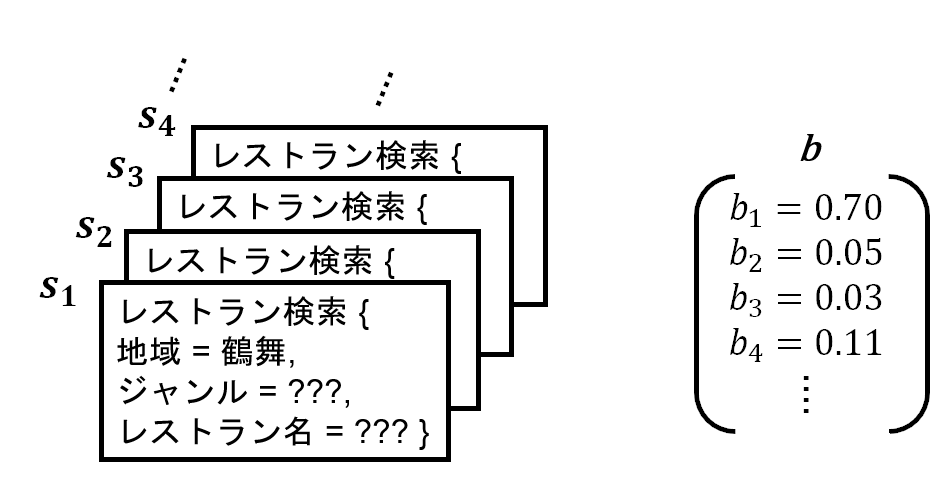
\includegraphics[width=10cm]{chapter2/belief.eps}
    \caption{対話状態の確率的表現である信念$b$ のイメージ図}
    \label{fig:belief}
  \end{center}
\end{figure}

統計的機械学習による対話状態追跡では,言語理解部からの誤りに対する頑健性を得るために,対話状態を確率的に扱う.これは,ユーザ発話の解釈に不確実性が存在するため,対話状態を直接観測できないとしているからである.対話状態の確率的表現は,全ての対話状態にわたる確率分布である信念 $b$ を用いる.信念に関する図を図\ref{fig:belief}に示す.また,言語理解部の出力はノイズを含むユーザ入力の観測 $o$ とし,対話状態の集合を$I_s$,システムの行動の集合を$K$とする.対話状態の推定は,ターン $t$ の対話状態を $s^t \in I_s$,
システムの対話行為を $a^t \in K$,観測状態を $o^t \in I_s$,ユーザの対話状態が$s$である信念(確率変数)を $b^t_s$ として,式\ref{joutai_suitei}を推定する問題となる.
\begin{equation}
  \label{joutai_suitei}
  b_s = P(s|o^{1:t})
\end{equation}
$P(s|o^{1:t})$ は,これまでの観測状態から推定した全てのユーザの対話状態にわたる確率分布である.つまり,履歴としてこれまでの観測状態を用いている.
\par
統計的機械学習による対話管理の一例として,部分観測マルコフ決定過程(Partially Observable Markov Decision Process ; POMDP)\cite{pomdp,pomdp_review}を用いた手法を説明する.POMDPベースのモデルは,信念状態の追跡と強化学習という2つのキーアイデアを組み合わせている\cite{pomdp_review}.
強化学習とは,システムの行動に対して報酬を与えることで,システムに報酬を最大化する行動を学習させるという機械学習の一種である.
\par

\begin{figure}[thb]
  \begin{center}
    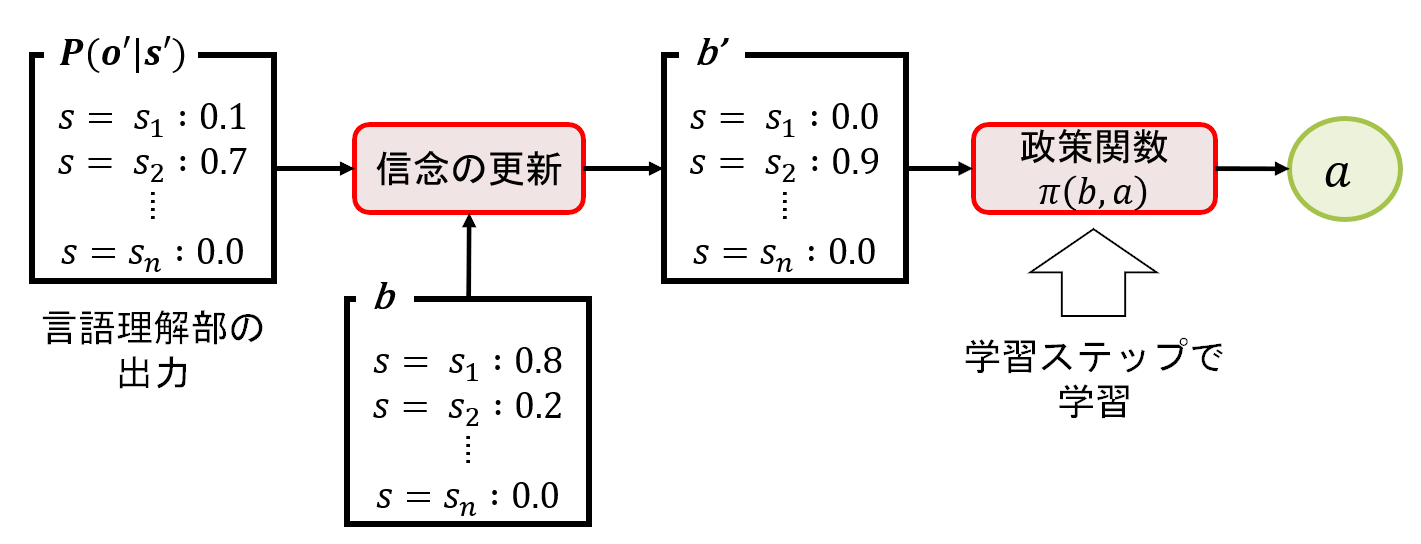
\includegraphics[width=15cm]{chapter2/pomdp2.eps}
    \caption{部分観測マルコフ決定過程(POMDP)の流れ}
    \label{fig:pomdp}
  \end{center}
\end{figure}


POMDPを用いた対話管理は図\ref{fig:pomdp}のように,言語理解部の出力を全ての対話状態にわたる確率分布 $p(o'|s')$ で表す.そして,信念状態の追跡には対話状態を最新の対話状態に更新する状態更新関数を用いる.状態更新関数は現在の対話状態 $s^{t+1}$ をこれまでの観測状態系列 $o^{1:t+1}$ から求める式である.状態更新関数は式\ref{state_update}に示す.
\begin{equation}
  \label{state_update}
  b' = P\left(s^{t+1}|o^{1:t+1}\right) \propto P\left(o'|s'_{j}\right) \Sigma_{s_i} P\left(s'_{j}|s_i, \widehat{a_k}\right)b^t
\end{equation}
式\ref{state_update} では,$P(o'|s'_j)$が観測確率,$P(s'_j|s_i,\widehat{a_k})$ が状態遷移確率,$b_t$が現在の信念を表す.
信念の更新をした後,状態 $s$ で対話行為 $a$ を選ぶ確率である政策関数$\pi (b,a)$を用いて次のシステムの対話行為を決める.POMDP での報酬は状態行動価値(Q値)などを用いる.Q 値とは,ある状態$s$のとき対話行為$a$を行い得られる報酬の期待値である.POMDPを用いた対話管理は,その報酬を用いて政策関数を強化学習により最適化していき,最適なシステムの対話行為を選ぶことを目指す.
\par
POMDPを用いた対話管理は,全ての状態にわたる信念の分布を維持することにより,システムは全ての可能な対話経路を効果的に並行して追求し,最も可能性の高い状態だけではなく,全ての状態にわたる確率分布に基づいて次の対話行為を選択することが可能になる\cite{pomdp_review}.
問題としては,複雑な対話を取り扱うと対話状態のパターンが増加するため,信念の追跡が困難になることがある.また,ルールベースほどではないが言語理解部の誤りにより性能が悪化する.